
Following from Lemma \ref{lem:transferdomination}, the current analysis studies the dual arm costs in the randomized unit tabletop setting, with $c_t$ as the cost measure per unit distance. 
For the $2$-arm setting, assume for simplicity that each arm's volume is represented as a disc of some radius 
$r$. For obtaining a $2$-arm solution, we partition the $n$ objects randomly 
into two piles of $\frac{n}{2}$ objects each; then obtain two initial solutions 
similar to the single arm case. It is expected (Eq.~\ref{eq:single-cost-simple}) that these two halves 
should add up to approximately $(c_{pd} + 0.52c_t)n$. 


\begin{theorem}
	\textit{For rearranging objects with non-overlapping starts and goals that are
	uniformly distributed in a unit square,  a $2$-arm solution can have an 
	asymptotic improvement of $\frac{1}{2}$ over the single arm solution. }
	\label{thm:karm}
\end{theorem}

\textit{Proof: }
From the initial $2$-arm solution, we construct an {\em asynchronous} $2$-arm 
solution that is collision-free. Assume that pickups 
and drop-offs can be achieved without collisions between the two arms, which 
can be achieved with properly designed end-effectors. The main overhead 
is then the potential collision between the two (disc) arms during transfer 
and move operations. Because there are $\frac{n}{2}$ objects for each arm to work 
with, an arm may travel a path formed by $n + 1$ straight line 
segments. Therefore, there are up to $(n + 1)^2$ intersections between the 
two end-effector trajectories where potential collision may happen. However,
because for the transfers and transits associated with one pair of objects (one 
for each arm) can have at most four intersections, there are at most 
$2n$ potential collisions to handle. For each intersection, let one 
arm wait while letting the other circling around it, which incurs a cost that is bounded by $2\pi \cdot
r \cdot c_t$. 


Adding up all the potential extra cost,  
% that a $2$-arm solution has 
a cumulative cost is obtained as 
% \begin{align}\label{eq:dual-cost-distance} 
% C_{dual} = C_{single} + 2n(2\pi rc_t) \approx (c_{pd} + 0.52c_t + 4\pi rc_t)n.
% \end{align}

{\centerline
{
$C_{\rm dual} = C_{\rm single} + 2n(2\pi rc_t) \approx (c_{pd} + 0.52c_t + 4\pi rc_t)n\;.$
}
}

\noindent For small $r$, $C_{\rm dual}$ is almost the same as $C_{\rm single}$ 
$c_t$ is a distance (e.g., energy) cost. Upon considering the maximum of the two arc lengths or makespan (Eq.~\ref{eq:cost_function}),
the $2$-arm cost becomes $C_{\rm dual}^t \approx (c_{pd} + 0.52c_t)\frac{n}{2} + 4n\pi rc_t$.
% \vspace{-0.1in}
% \begin{equation}\label{eq:dual-cost-time}
% C_{dual}^t \approx (c_{pd} + 0.52c_t)\frac{n}{2} + 4n\pi rc_t
% \vspace{-0.1in}
% \end{equation}
% {\centerline
% {
% $C_{dual}^t \approx (c_{pd} + 0.52c_t)\frac{n}{2} + 4n\pi rc_t$
% }
% }
The cost ratio is
%\vspace{-0.1in}
\begin{align*}\label{eq:makespan-ratio}
\frac{C_{\rm dual}^t}{C_{\rm single}} &\approx 
\frac{(c_{pd} + 0.52c_t)\frac{n}{2} + 4n\pi rc_t}{(c_{pd} + 0.52c_t)n}
\\&= \frac{1}{2} + \frac{4\pi rc_t}{c_{pd} + 0.52c_t}\;.\numberthis
% \vspace{-0.1in}
\end{align*}



\commentdel{
 \begin{wrapfigure}{r}{1.4in}
%  \vspace{-.45in}
	\centering
    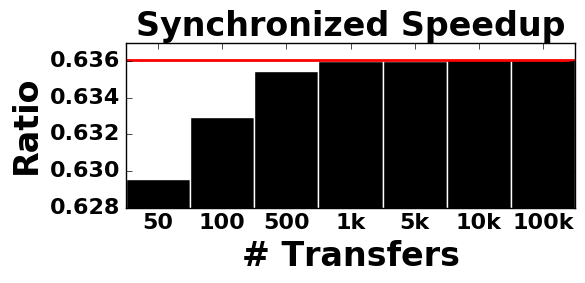
\includegraphics[width=1.4in]{figures/monte_carlo}
%    \vspace{-.4in}
	\caption{Empirical cost ratio versus the estimate}
  	\label{fig:bounds}
%    \vspace{-.4in}
\end{wrapfigure}
}

When $r$ is small or when $\frac{c_t}{c_{pd}}$ is small, the $2$-arm 
solution is roughly half as costly as the single arm solution. On 
the other hand, in this model a $2$-arm solution does not do better than $\frac{1}{2}$ of 
the single arm 
solution. $ \qed $

%This argument can be extended to $k$-arms as well \cite{Shome2018WAFR}.



%\vspace{-0.08in}
\commentadd{
%\begin{theorem}
%For rearranging objects with non-overlapping starts and goals that are
%uniformly distributed in a unit square,  a $2$-arm solution can have an 
%asymptotic improvement of $\frac{1}{2}$ over the single arm solution. 
%\label{thm:karm}
%\end{theorem}
}


\tase{
\begin{theorem}
	\textit{For rearranging objects with non-overlapping starts and goals that are
	uniformly distributed in a unit square,  a $k$-arm solution can have an 
	asymptotic improvement of $\frac{1}{k}$ over the single arm solution. }
\end{theorem}

\textit{Proof:}	
%\subsection{Expected k-arm cost bounds in a planar disk manipulator model}
\commentadd{The arguments made in Theorem \ref{thm:karm} can be extended to $k$ disc arms.
	In the planar unit-square setting, with $k$ arms, there are $\frac{n}{k}$ objects 
	for each arm to work with. Consider the transfers and transits of a set of $k$ 
	objects, one for each arm. By \cite{ChiHanYu2018WAFR}, the arbitrary rearrangement of $k$ discs 
	can be achieved in a bounded region with a perimeter of $O(kr)$. 
	Clearly, the per robot additional (makespan or distance) cost is bounded by some 
	function $f(k, r)c_t$, which goes to zero as $r$ goes to zero. Adding up all the potential 
	extra cost,  a $k$-arm solution has a cumulative cost
	
	{\centerline
		{
			$C_{\rm k{\text-}arm} = C_{\rm single} + nf(k,r)c_t \approx (c_{pd} + 0.52c_t + f(k,r)c_t)n\;.$
		}
	}
	
	\noindent For fixed $k$ and small $r$, $C_{\rm k{\text-}arm}$ is almost the same as $C_{\rm single}$.
	%, $c_t$ is a distance (e.g., energy) cost. 
	Upon considering the maximum of the two arc lengths or makespan,
	the $k$-arm cost becomes $C_{\rm k{\text-}arm}^t \approx (c_{pd} + 0.52c_t)\frac{n}{k} + nf(k,r)c_t$.
	
	The cost ratio is
	\vspace{-0.1in}
	\begin{align*}\label{eq:kmakespan-ratio}
	\frac{C_{\rm k{\text-}arm}^t}{C_{\rm single}} &\approx 
	\frac{(c_{pd} + 0.52c_t)\frac{n}{k} + nf(k,r)c_t}{(c_{pd} + 0.52c_t)n}
	\\&= \frac{1}{k} + \frac{f(k,r)c_t}{c_{pd} + 0.52c_t}\;.\numberthis
	% \vspace{-0.1in}
	\end{align*}
	
	When $r$ is small or when $\frac{c_t}{c_{pd}}$ is small, the $k$-arm 
	solution is roughly $\frac{1}{k}$ as costly as the single arm solution. On 
	the other hand, in this model a $k$-arm solution does not do better than $\frac{1}{k}$ of 
	the single arm. \qed
	
%	\begin{theorem}
%		For rearranging objects with non-overlapping starts and goals that are
%		uniformly distributed in a unit square,  a $k$-arm solution can have an 
%		asymptotic improvement of $\frac{1}{k}$ over the single arm solution. 
%	\end{theorem}
}
% \rahul{Need to verify this line of reasoning}

}


\begin{theorem}
	\textit{For rearranging objects with non-overlapping starts and goals that are 
	uniformly distributed in a unit square,  a randomized $2$-arm \textit{synchronized} solution can have an 
	asymptotic improvement of $\frac{1}{2}$ over the single arm solution if $\frac{c_t}{c_{pd}}$ is small, and a improvement $\approx 0.64$ when both $c_{pd}$ and $r$ are small. }
\end{theorem}


\textit{Proof:} The synchronization assumption changes the expected cost of the solution. The random partitioning of the $n$ objects into two sets of $\frac{n}{2}$ object with a random ordering of the objects yields $\frac{n}{2}$ pairs of objects transfers, which dominate the total cost for large $n$. The cost~(Eq.~\ref{eq:cost_function}) of $\frac{n}{2}$ synchronized transfers ($\coma_i$) includes $\frac{n}{2}c_{pd}$ and $C^{\rm sync}_{sg} \approx (\mathtt{E}(max(l_1,l_2))c_t)\frac{n}{2}$, where $\mathtt{E}(max(l_1,l_2))$ is the expected measure of the max of lengths $l_1$,$l_2$ of two randomly paired transfers. Using the \textit{pdf}\cite{ghosh1951random} of lengths of random lines in an unit square and integrating over the setup\cite{Shome2018WAFR}, results in the value of $\mathtt{E}(max(l_1,l_2))$ to be $0.66$ . 
% (Section \ref{sec:appendix}). 



\tase{
\begin{lemma}
	Expected measure of the maximum of lengths of two random lines on an unit square is $ 0.66 $.
\end{lemma}

\textit{Proof:} Prior work \cite{ghosh1951random} defines the \textit{probability distribution function (pdf)} of lengths($l$) of randomly sampled lines in a rectangle.
% of sides $a,b, \ \ a\geq b$.
% as 
%\begin{align*}
%p(l) &= (\frac{4l}{a^2b^2})\phi(l)\\
%\phi(l)&= \frac{1}{2}\pi a b - a l - b l + \frac{1}{2} l^2, \ \ l\in[0,b]\\
%\phi(l)&= ab \sininv(\frac{b}{l}) + a. \sqrt[]{(l^2-b^2)} - al - \frac{1}{2}b^2, \ \ l\in[b,a]\\
%\phi(l)&= ab\{\sininv(\frac{b}{l})-\cosinv(\frac{a}{l})\} + a\sqrt[]{(l^2-b^2)} + b\sqrt[]{(l^2-a^2)} \\
%&- \frac{1}{2}(l^2+a^2+b^2),\ \ l\in[a,\sqrt[]{(a^2+b^2)}]
%\end{align*}

%In the unit square model, $a=b=1$. Substituting the values, the \textit{pdf} becomes
In the unit square model, substituting the values for the dimensions of the sides of the rectangle with $1$, the \textit{pdf} can be simplified as follows.
\begin{align*}
p(l)&= 2\pi l - 8\pi l^2 + 2l^3, \ \ l\in[0,1]\\
p(l)&= 4l\sininv(\frac{1}{l}) - 4l\cosinv(\frac{1}{l}) + 8l\sqrt[]{(l^2-1)} -2l^3 -4l,\\ &\ l\in[1,\sqrt[]{2}]
\end{align*}

Assuming two random sets of lines, representing transfers in a random split of objects between two arms, we need the expected value of the maximum of these pairwise lengths ie., $\mathtt{E}(max(l_1,l_2)), \ \ l_1,l_2\ i.i.d, \ \ l_1 \sim p, l_2 \sim p$.
This is estimated using the \textit{pdf} obtained. 
\begin{align*}
\mathtt{E}(max(l_1,l_2)) &= \int_0^{\sqrt[]{2}} \int_0^{\sqrt[]{2}} max(l_1,l_2)p(l_1)p(l_2) dl_2 dl_1\\&\approx 0.663
\end{align*}
The result is calculated by taking into account the combination of different ranges of $p(l)$ and $max(l_1,l_2)$.
\commentadd{
%	\begin{figure}[h]
%		\centering
%		%	\vspace{-0.3in}
%		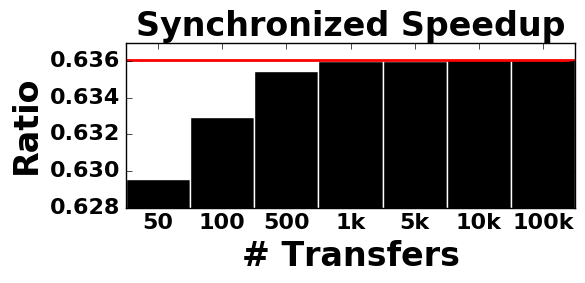
\includegraphics[width=0.35\textwidth]{figures/monte_carlo}
%		\caption{Empirical cost ratio versus the estimate}
%		\label{fig:mcbounds}
%	\end{figure}
	
	Prior work~\cite{santalo2004integral} offered an estimate for the expected length of a transit path $C_{sg}$ in terms of the expected length of a line segment, $0.52$, in a randomized setting in an unit square. With the current estimate of $0.663$ for the maximum of two such randomly sampled line segments, it follows that, the expected makespan or maximum of distances cost will use this estimate.\qed
	
%	Using this result, the synchronized cost ratio is stated in Equation~\ref{eq:synchronized-ratio} as
%	$$
%	\frac{C_{\rm dual}^{\rm sync}}{C_{\rm single}} \approx 
%	\frac{(c_{pd} + 0.66c_t)\frac{n}{2} + 4n\pi rc_t}{(c_{pd} + 0.52c_t)n}
%	$$
%	As a way to validate our asymptotic estimate, randomized trials were run with different number randomly sampled object transfer coordinates on an unit square.
%	% Fig \ref{fig:bounds} verifies empirically that the ratio of $\frac{C_{dual}^{sync}}{C_{single}}$ when $c_{pd}=0,r=0$, asymptotically converges to the calculated expected value of $0.636$. 
%	When $c_{pd}=0$ and $r=0$, the ratio of $\frac{C_{dual}^{sync}}{C_{single}}$ evaluates to $0.636$. Fig \ref{fig:mcbounds} verifies empirically that the ratio converges to the expected value as the number of transfers increases.
%	This indicates the asymptotic speedup of a synchronized dual arm solution for a makespan or maximum of distances cost metric.
}

}

This means $C_{\rm dual}^{\rm sync} \approx (c_{pd} + 0.66c_t)\frac{n}{2} + 4n\pi rc_t$.
% \vspace{-0.1in}
% \begin{equation}\label{eq:synchronized-cost}
% C_{dual}^{sync} \approx (c_{pd} + 0.66c_t)\frac{n}{2} + 4n\pi rc_t
% \vspace{-0.1in}
% \end{equation}
% {\centerline
% {
% $C_{dual}^{sync} \approx (c_{pd} + 0.66c_t)\frac{n}{2} + 4n\pi rc_t$
% }
% }
The synchronized cost ratio is
%\vspace{-0.1in}
\begin{align*}\label{eq:synchronized-ratio}
\frac{C_{\rm dual}^{\rm sync}}{C_{\rm single}} &\approx 
\frac{(c_{pd} + 0.66c_t)\frac{n}{2} + 4n\pi rc_t}{(c_{pd} + 0.52c_t)n}
\\&= \frac{1}{2} + \frac{ (0.07 + 4\pi r)c_t}{c_{pd} + 0.52c_t}\;.\numberthis
%\vspace{-0.1in}
\end{align*}

When $\frac{c_t}{c_{pd}}$ is small, even the synchronized $2$-arm solution provides an improvement of $\frac{1}{2}$. For the case when both $r$ and $c_{pd}$ are small, we observe that the ratio approaches $0.636$. 
\commentdel{Fig \ref{fig:bounds} confirms empirically that in randomized trials on an unit square, the ratio of $\frac{C_{dual}^{sync}}{C_{single}}$ when $c_{pd}=0,r=0$, converges to the calculated estimate (red line).}

\tase{
	\begin{figure}[h]
		\centering
		%	\vspace{-0.3in}
		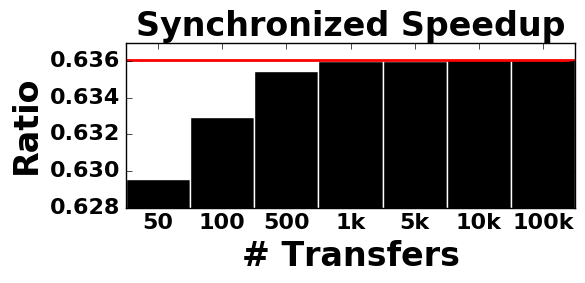
\includegraphics[width=0.35\textwidth]{figures/monte_carlo}
		\caption{Empirical cost ratio versus the estimate}
		\label{fig:mcbounds}
	\end{figure}
	As a way to validate our asymptotic estimate, randomized trials were run with different number randomly sampled object transfer coordinates on an unit square.
% Fig \ref{fig:bounds} verifies empirically that the ratio of $\frac{C_{dual}^{sync}}{C_{single}}$ when $c_{pd}=0,r=0$, asymptotically converges to the calculated expected value of $0.636$. 
When $c_{pd}=0$ and $r=0$, the ratio of $\frac{C_{dual}^{sync}}{C_{single}}$ evaluates to $0.636$. Fig \ref{fig:mcbounds} verifies empirically that the ratio converges to the expected value as the number of transfers increases.
This indicates the asymptotic speedup of a synchronized dual arm solution for a makespan or maximum of distances cost metric.
}

\qed
%\vspace{-0.08in}
%\begin{theorem}
%For rearranging objects with non-overlapping starts and goals that are 
%uniformly distributed in a unit square,  a randomized $2$-arm synchronized solution can have an 
%asymptotic improvement of $\frac{1}{2}$ over the single arm solution if $\frac{c_t}{c_{pd}}$ is small, and a improvement $\approx 0.64$ when both $c_{pd}$ and $r$ are small. 
%\end{theorem}


\commentadd{
\noindent \textbf{Note on bounds:} Even though the proposed simplified model does not apply immediately costs and collision volumes in general configuration spaces, experiments indicate that the speedups exist in these spaces as well.
}
% \rahul{this paragraph is phrased contradictorily. It makes sense if the first sentence is for asynchronous cases.}
% We note that the same can be said for a {\em synchronous} $2$-arm solution if
% when $c_t/c_{pd}$ is small. 
% Under the synchronization assumption, $C_{dual}^t$
% is no longer necessarily expected to be $\frac{C_{single}}{2}$ for large $n$. 
% Experiments in the next section indicate that improvements over single arm solutions in practical settings.

%\textcolor{red}{NOTE: We can also generate plots illustrating how the ratio 
%change as $n$, $r$, $c_{pd}:c_t$ changes. We may also further generalize the 
%$r$ based collision term to a more general collision term.}


%\begin{figure}[h]
%%  \begin{center}
%\centering
%    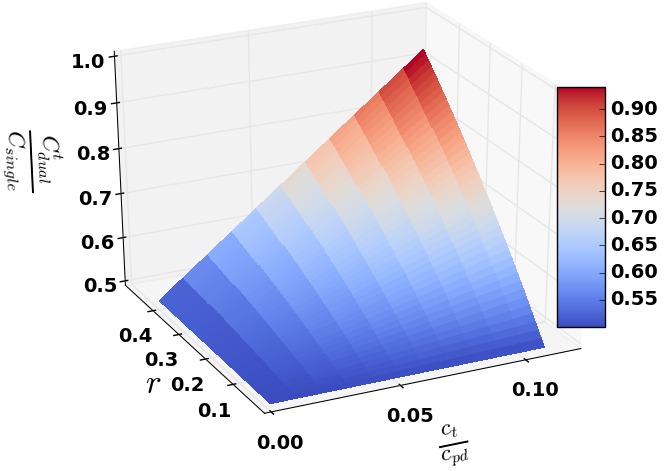
\includegraphics[width=2in]{figures/bounds}
%%  \end{center}
%  \caption{Bounds}
%  	\label{fig:bounds}
%\end{figure}


